% Appendix

\chapter*{Appendix A} % Main appendix title

\label{AppendixA} % Change X to a consecutive letter; for referencing this appendix elsewhere, use \ref{AppendixX}

\begin{figure}
      \centering
      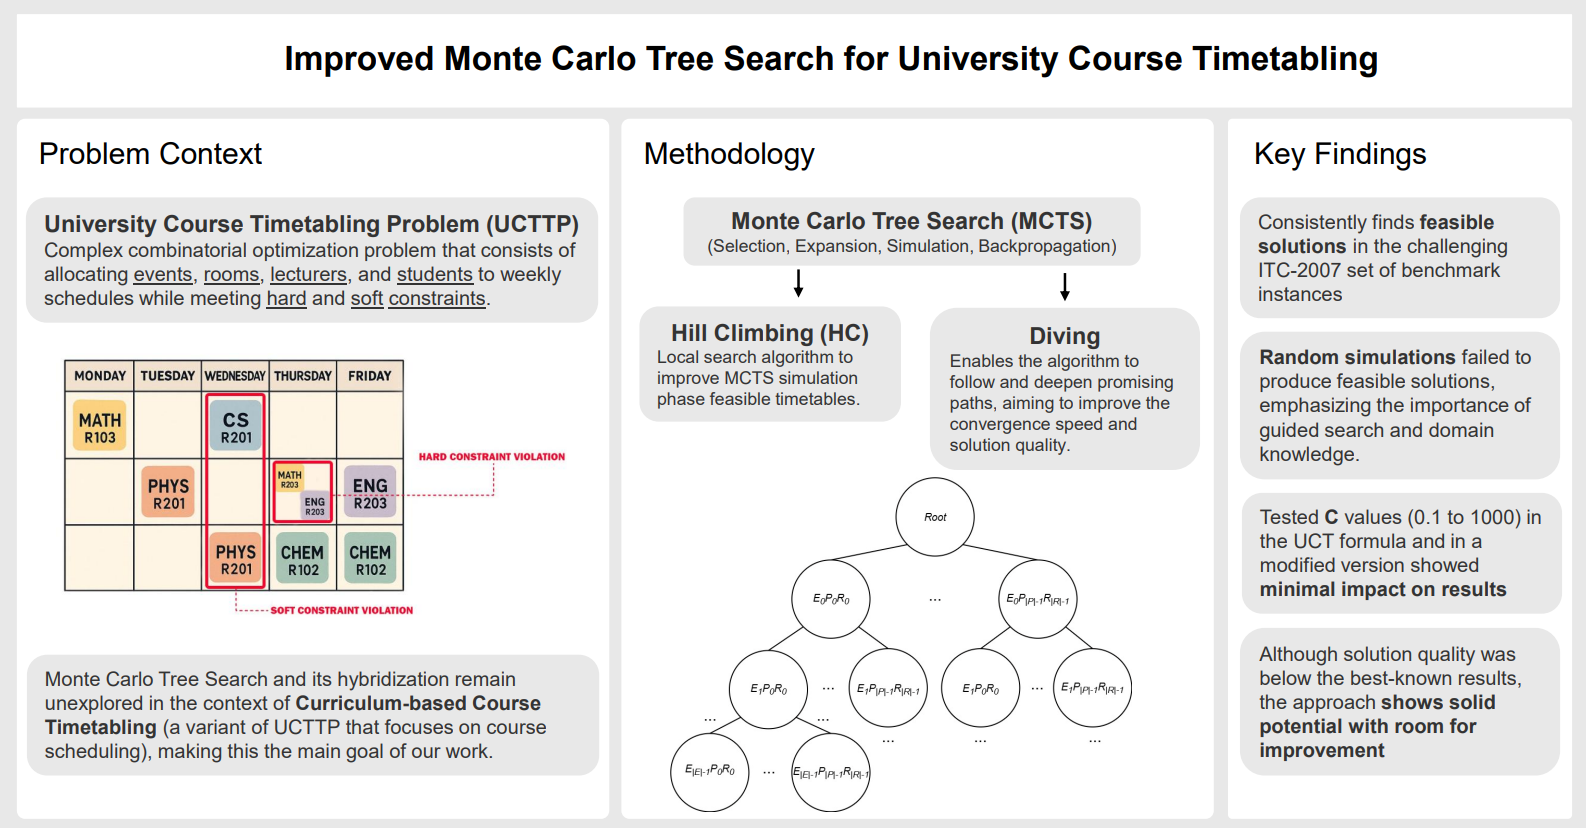
\includegraphics[width=1.0\columnwidth]{AppendixA/graphical_abstract.png}
      \caption[Proposed \ac{mcts} tree]
      {Graphical abstract illustrating the problem context, proposed methodology, and key findings of this dissertation.}
      \label{fig:graphical_abstract}
\end{figure}

\begin{figure}
      \centering
      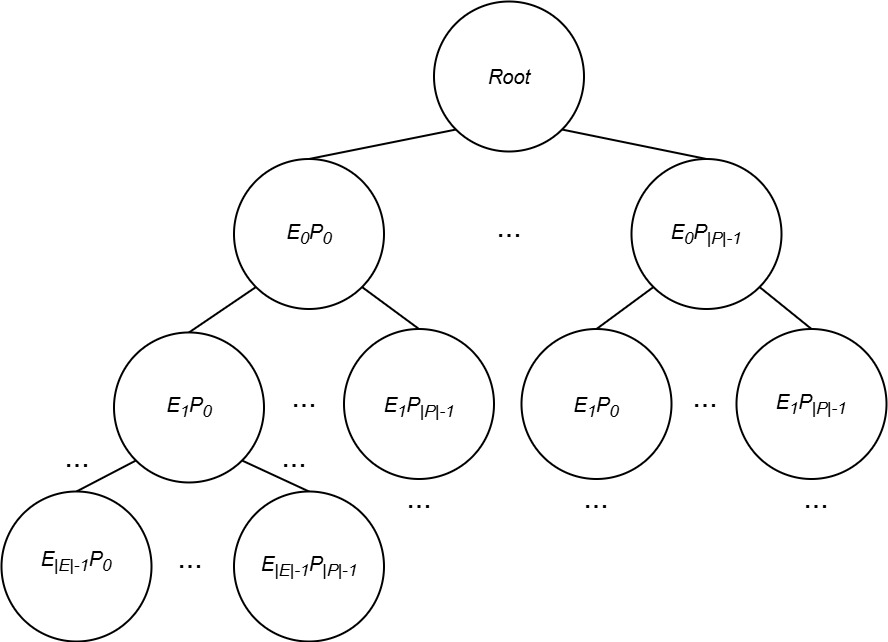
\includegraphics[width=0.7\columnwidth]{AppendixA/tree.jpg}
      \caption[Proposed \ac{mcts} tree]
      {Proposed \ac{mcts} tree}
      \label{fig:tree}
\end{figure}


\begin{figure}
      \centering
      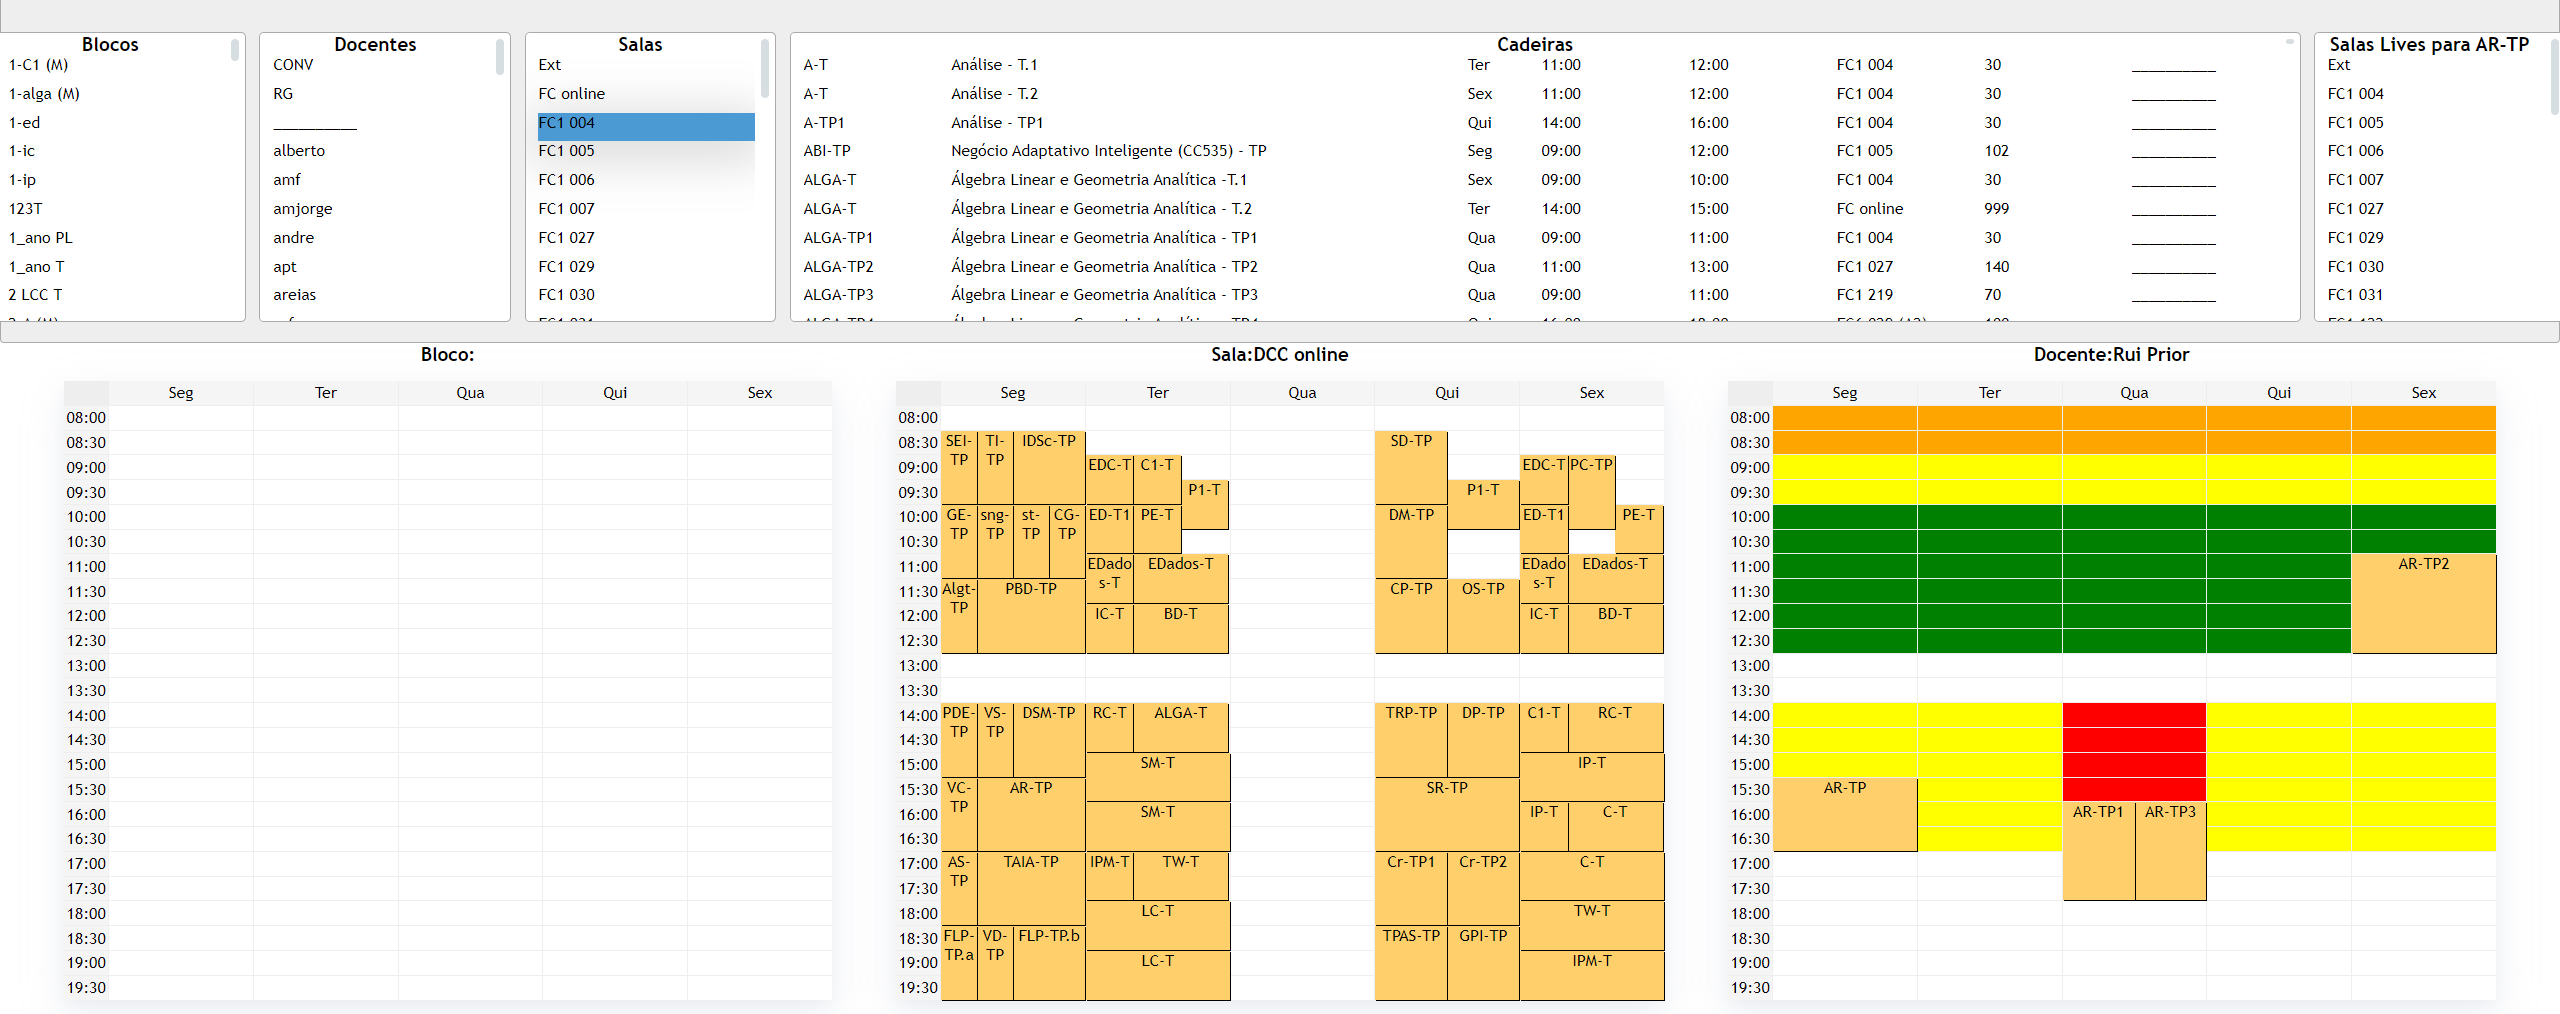
\includegraphics[width=1.0\columnwidth]{AppendixA/previous_work.png}
      \caption[Previous work interface]
      {Previous work interface}
      \label{fig:previous_work_interface}
\end{figure}

\begin{figure}
      \centering
      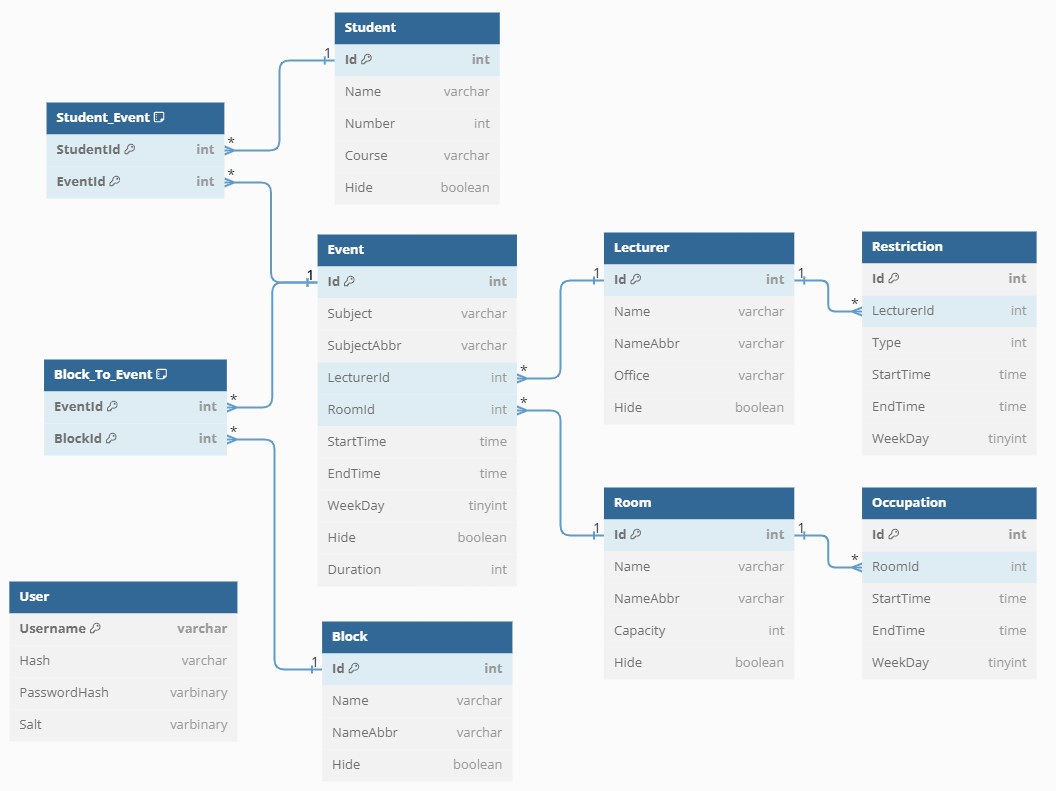
\includegraphics[width=1.0\columnwidth]{AppendixA/uml.png}
      \caption[Previous work UML]
      {Previous work UML}
      \label{fig:previous_work_uml}
\end{figure}

\vspace*{10cm}
\newfontfamily\sinhalaFont{Nirmala UI}
\tikz[baseline]{
  \node[opacity=0.05, text=black, font=\sinhalaFont] at (0,0) {ඞ};
}